\documentclass[class=scrbook, crop=false]{standalone}
\usepackage[subpreambles=true]{standalone}
\ifstandalone
    % WARNING: Proceed with caution!

% -----------------------------------------------------------------------------------
% For package standalone
% -----------------------------------------------------------------------------------
\usepackage{import}

% -----------------------------------------------------------------------------------
% Language and typeset
% -----------------------------------------------------------------------------------
\usepackage[ngerman, english]{babel}

\usepackage{subcaption}
% Umlauts and other special characters (UTF-8)
% \usepackage[utf8]{inputenc}
\usepackage{fontspec}
\setsansfont{Arial}
% \usepackage[T1]{fontenc}  % Enable accented characters and umlauts
% LuaLatex doesn't need fontenc and uses UTF-8
% \usepackage{lmodern}  % Font face


% --------------------------------------------------------------------------------
% Page formatting
% --------------------------------------------------------------------------------
% Change the header/footer for chapter beginnings and normal pages
\usepackage[automark,headsepline]{scrlayer-scrpage}

% The package provides an easy and flexible user interface to customize the page
% layout, implementing auto-centering and auto-balancing mechanisms
% WARNING: WHEN CHANGING BCOR (Binding correction), the cover needs reworking!...
\newcommand{\theBCOR}{15mm}  % Define binding correction
\usepackage[
    bindingoffset=\theBCOR,
    % showframe, % Show boxes which indicate margins and paddings
    bottom = 3.5cm, % Margins
      left = 2.5cm,
     right = 2.5cm
] {geometry}

% The package 'float' provides a container for document objects which can not be
% broken over pages, such as tables and figures
% Needed for table and figure indexes  
\usepackage{float}

% support for landscape layout
\usepackage{lscape}

% support of \tablenotes command to add notes under table
\usepackage{threeparttable}

% To allow drawing more professional tables
\usepackage{booktabs}

% --------------------------------------------------------------------------------
% Contents
% --------------------------------------------------------------------------------
% Vector graphics (for Cover page)
\usepackage{tikz} 

% Allows additional parameters when including images
\usepackage{graphicx}

% Roman font family for all headings
\addtokomafont{disposition}{\rmfamily}

% Set the line spacing to 1.5
\usepackage[onehalfspacing]{setspace}

% Improves overall text spacing
% http://www.khirevich.com/latex/microtype/
\usepackage[stretch=10]{microtype}

% Math symbols like mu outside the math environment
\usepackage{textcomp}

% A comprehensive (SI) units package∗
% For defining SI units
\usepackage[
    range-units=single,         % Formatting ranges with single unit indication: 1 - 2 m
    range-phrase=-,             % Phrase for range: 1 - 2 m vs 1 to 2 m
    separate-uncertainty=true,  % sets +- between value and uncertainty 
    multi-part-units=repeat     % In expressions with multiple values (multi part numbers) 
                                % the unit is printed each time: 1 mm x 1 mm
] {siunitx}
% https://tex.stackexchange.com/questions/124488/multi-part-numbers-and-units-in-siunitx

% Allows Sourcecodes with highlighting 
\usepackage{listings}

% This package provides user control over the layout of the three basic list
% environments: enumerate, itemize and description
\usepackage{enumitem}
\setlist{nosep} % Remove the vertical space between \item elements in all lists

% ToDo Notes
% \setlength{\marginparwidth}{2cm}
\usepackage{todonotes}
\setuptodonotes{inline, inlinepar}
\reversemarginpar  % Put ToDo notes on the binding's side
% \usepackage{soul} % Colorful ToDo notes

% Check out colors here http://latexcolor.com/
\usepackage{xcolor}

\usepackage{amsmath}    % alignment of equations

% --------------------------------------------------------------------------------
% Other elements
% --------------------------------------------------------------------------------
% Blindtext: Organic looking text dummy
\usepackage{blindtext}

% Hyperlinks within the document (PDF)
% "hidelinks" hides visual highlighting of links
\usepackage[hidelinks]{hyperref}

% Package for Glossary and Index (Acronyms are listed in a separate list) 
\usepackage[acronym, nogroupskip]{glossaries}[=v4.49] % groupskip: alphabetic grouping of entries

\usepackage{xltabular}   % <------- FOR glossaries

% Integration and management of bibliographies
\usepackage{csquotes}   % backend=biber in biblatex needs this package
\usepackage[
    style=ieee,   % style of the bibliography, entries are sorted in alphabetic order. "ieee" is another common style.
    backend=biber,      % based on package 'biber' 
    bibencoding=ascii   % ASCII Text encoding; may use "utf8" instead
] {biblatex}

% --------------------------------------------------------------------------------
%                               PATHS & FILES
% --------------------------------------------------------------------------------
% Fix paths for standalone compiling
\ifstandalone
    \def \home {..}
\else
    \def \home {.}
\fi

% Package: scrlayer-scrpage
% \def \stylePath {\home/settings+/style/page}
\input{\home/settings+/style/page}  % Load page style

% Package: graphicx
\graphicspath{{\home/images/}}  % Set path to images

% Package: listings
\input{\home/settings+/style/code.tex}  % Set path to style file
\lstset{inputpath={\home/code/}} % Default path to code listings

% Package: glossaries
\input{\home/settings+/style/symbols}  % Set path to symbols list style file
\input{\home/settings+/style/acronyms}  % Set path to acronym list style file
% -------------------------------------------------------------------------------
%               Listing of all Glossary and Acronym Entries 
%                           use as shown below
% -------------------------------------------------------------------------------

% ==== EXEMPLARY ENTRY FOR SYMBOLS LIST =========================================

% ==== EXEMPLARY ENTRY FOR ACRONYMS LIST ========================================
% \newacronym{#label}{#acronym}{#long_form}

% define new command for custom arconym entry with only two arguments
% fabricates an easier way to use \newacronym 
\newcommand{\acroX}[2]{\newacronym{#1}{#1}{#2}}
% \acroX{label and arconym}{long name}
% \acroX{CD}               {Compact Disk}

\newcommand{\acroY}[3]{\newacronym{#1}{#2}{#3}}
% \arcoY{label}{acronym}{long name}
% \acroY{CD}   {cd}     {Compact Disk}
 
\newacronym{AEP}{AEP}{Imbalance price}
\newacronym{aFRR}{aFRR}{Automatic Frequency Restoration Reserve}


\newacronym{reBAP}{reBAP}{Uniform imbalance price}
\newacronym{TSO}{TSO}{Transmission System Operator}
\newacronym{FCR}{FCR}{Frequency Containment Reserve}
\newacronym{mFRR}{mFRR}{Manual Frequency Restoration Reserve}
\newacronym{BRP}{BRP}{Balancing Responsible Party}
\newacronym{SB}{SB}{System Balance}
\newacronym{VRE}{VRE}{variable renewable energy}
\newacronym{ID1}{ID1}{intraday index ID1}
\newacronym{MAE}{MAE}{mean average error}
\newacronym{RMSE}{RMSE}{root mean squared error}
\newacronym{MSE}{MSE}{mean squared error}
\newacronym{CRPS}{CRPS}{continuous ranked probabililty score}
\newacronym{GCC}{GCC}{Grid Control Cooperation}
\newacronym{IC}{IC}{Continuous intraday}
\newacronym{VWAP}{VWAP}{volume-weighted average price}
\newacronym{VID}{VID}{traded volume within the intraday market}
\newacronym{ID AEP}{ID AEP}{Intraday Average Energy Price}
\newacronym{FRR}{FRR}{Frequency Restoration Reserve}
\newacronym{TFT}{TFT}{Temporal Fusion Transformer}
\newacronym{DLM}{DLM}{Dynamic Linear Model}
\newacronym{GB}{GB}{Gradient Boosting}
\newacronym{RF}{RF}{Random Forest}
\newacronym{ARIMAX}{ARIMAX}{Autoregressive Integrated Moving Average with eXogenous variables}
\newacronym{xLSTM}{xLSTM}{Extended Long Short-Term Memory}
\newacronym{DWD}{DWD}{Deutscher Wetterdienst}
\newacronym{ENTSO-E}{ENTSO-E}{European Network of Transmission System Operators for Electricity}
\newacronym{IDA1}{IDA1}{Intraday auction 1}
\newacronym{MOSMIX}{MOSMIX}{Model Output Statistics-MIX}
\newacronym{mLSTM}{mLSTM}{memory-optimized LSTM}
\newacronym{sLSTM}{sLSTM}{speed-optimized LSTM}

% ==== EXEMPLARY ENTRY FOR MAIN GLOSSARY ========================================

    % \newglossaryentry{policy}{name={Policy},description={Im geschäftlichen Bereich bezeichnet Policy eine interne Leit- bzw. Richtlinie, die formal durch das Unternehmen dokumentiert und über ihr Management verantwortet wird}}
    % \newglossaryentry{pcie}{name={PCI Express},description={PCI Express („Peripheral Component Interconnect Express“, abgekürzt PCIe oder PCI-E) ist ein Standard zur Verbindung von Peripheriegeräten mit dem Chipsatz eines Hauptprozessors. PCIe ist der Nachfolger von PCI, PCI-X und AGP und bietet im Vergleich zu seinen Vorgängern eine höhere Datenübertragungsrate pro Pin.}}
    % \newglossaryentry{realnumber}
  % Load glossary, symbol and acronyms list

% Package: biblatex
\addbibresource{\home/references/references.bib}  % Set path to bib resources

% Custom variables
\input{\home/settings+/variables}
% --------------------------------------------------------------------------------
%                                   OPTIONAL
% --------------------------------------------------------------------------------


% Simple arithmetic for LaTeX commands
% \usepackage{calc}

% Document Elements
% -------------------

% Index
% \usepackage{imakeidx}

% compact Lists
%\usepackage{paralist}

% visual improvements for citations
% \usepackage{epigraph}

% Create pseudo code
% https://www.overleaf.com/learn/latex/Algorithms
% \usepackage{algorithm}
% \usepackage{algorithmic}
%\usepackage[noend]{algpseudocode}

% Formatting
% -------------------
% Tweaks for scrbook, redefines commands of other packages
% \usepackage{scrhack}

% Intelligent space separator (nice for superscript?)
% \usepackage{xspace}

% Allows breaks within tables
%\usepackage{tabularx}

% Allows for page breaks in tables
% \usepackage{longtable}

% allows modifying of captions
% \usepackage{caption}

% Multiline comments
%\usepackage{verbatim}

% % Custom colors
% \definecolor{dartmouthgreen}{rgb}{0.05, 0.5, 0.06}

% IF you want to define unicode characters
% \DeclareUnicodeCharacter{0229}{\c{e}}
% \DeclareUnicodeCharacter{0306}{\u{Z}}


% Document elements
% ------------------------------------

% Table package
% \usepackage{booktabs}

% Pie diagram
% \usepackage{datapie}

% Side by Side images
% \usepackage{subcaption}

% For landscape tables
%\usepackage{pdflscape}
%\usepackage{afterpage}

% Graphics can be flow around by text
%\usepackage{wrapfig}

\fi

% ----------------------------------------------------------------------------
%                               Discussion
% ----------------------------------------------------------------------------
\begin{document}

\chapter{Results and Discussion} % Overview text
\label{Chapter::Results and Discussion}
In this chapter, the results of the thesis are discussed. The following sections contain th results of the experiments specified in \ref{Chapter::Experiments}.                   
    In this chapter, the results of the thesis are presented and evaluated as well as, the approach of this thesis.

% Show your results and analyze them
% Explain why the results are the way they are and not different
% Go into possible measurement errors and why they occurred
% Look for anomalies and explain why they occur
\section{Results}
\label{Section::Results}

\section{Out of the box performance}

The comparison of out-of-the-box model performance (Tables \ref{Table::Out_of_the_box_performance} and \ref{Table::Out_of_the_box_performance_quantile}) highlights clear differences in how each approach handles point forecasting, probabilistic estimation, and tail risk.

The xLSTM model achieves the strongest overall performance, with the lowest MAE (84.33), outperforming the naive ID1, and lowest CRPS (40.30) across all models. It also performs competitively in RMSE (302.57), suggesting that it not only captures average-case dynamics reliably, but also handles larger deviations effectively.

The iTransformer, by contrast, achieves the lowest RMSE (200.19), suggesting strong sensitivity to extreme price events. However, it exhibits the highest MAE (139.87) and CRPS (49.24), which points to less stable average-case performance and weaker calibration. Notably, its coverage rates are the highest across all models (e.g. 98\%-coverage of 0.959).

The Random Forest model provides solid baseline performance, with a relatively low MAE (99.00) and the second-best CRPS (41.37). Its RMSE (353.81) is notably higher, indicating reduced robustness to extreme values. Nevertheless, its prediction intervals are among the most reliable in the mid quantiles, with strong 90\%- and 98\%-coverage.

The ARIMA model performs similarly to Random Forest in terms of MAE (100.50) and CRPS (42.04), but has the highest RMSE (358.75) among all models, suggesting that it fails to capture large price spikes — a known limitation of linear, autoregressive models.

As shown in Figure \ref{Figure::pinball_scores}, the iTransformer achieves the lowest normalized pinball loss at the 90th percentile, highlighting their strength in forecasting extreme imbalance price events. This suggests that this model is well-suited to anticipating high-price outliers, which aligns with their superior RMSE compared to the other models.
In contrast, Random Forest, ARIMA and xLSTM perform better in the lower and mid quantiles, aligning with their lower MAE and CRPS. These models offer more accurate average-case predictions, but struggle with extreme events, which limits their effectiveness in capturing tail risk.

Compared to the naive ID1 benchmark, the trained models show mixed performance. While Random Forest, ARIMA and xLSTM outperform ID1 in CRPS, and iTransformer in RMSE, only xLSTM achieves a lower MAE than ID1.
However, when it comes to prediction interval coverage, all models surpass the benchmark significantly, with iTransformer achieving the best 50\%, 90\%, and 98\% coverage among all models.

These results support the thesis hypothesis: modern deep learning models can outperform classical methods and naive market heuristics, particularly for tail risks. However, Random Forest proves highly competitive—offering robust performance without the need for extensive tuning or sequence modeling.


  
  \begin{table}[]
\centering
\begin{tabular}{l|l|l|l}
Model name 		&  RMSE 			& MAE 			& CRPS 			\\\hline
Naive intraday ID1 	&$ 308.69 			$&$ 93.17 			$&$ 42.90			$ \\
Random forest 		&$ 353.81 \pm 0.19	$&$  99.00	\pm 0.17	$&$ 41.37 \pm 0.06	$\\
Arima 			&$ 358.75 			$&$ 100.50 		$&$ 42.04  			$\\	
iTransformer 		&$ \underline{200.19 \pm 0.07}	$&$ 139.87	\pm 0.06	$&$ 49.24 \pm 0.04	$ \\
xLSTM 			&$ 302.57\pm 6.68	$&$ \underline{84.33 \pm 1.17}	$&$ \underline{40.30	\pm0.24} $\\
\end{tabular}
\caption{Error metrics and CRPS for out of the box performance}
\label{Table::Out_of_the_box_performance}
\end{table}
\begin{table}
\centering
\begin{tabular}{l|l|l|l}
Model name 		&  50\%-cov 		& 90\%-cov 		& 98\%-cov \\\hline
Naive intraday ID1 	&$ 0.084			$&$ 0.557 			$&$ 0.844			$ \\
Random forest 		&$ 0.147 \pm0.003	$&$ 0.772\pm 0.007	$&$ 0.945	 \pm 0.005	$\\
Arima 			&$ 0.211			$&$ 0.612	 		$&$0.810 			$\\	
iTransformer 		&$ \underline{0.356	\pm 0.001}	$&$ \underline{0.841	\pm 0.000}	$&$ \underline{0.959 \pm 0.000}	$ \\
xLSTM 			&$ 0.240 \pm 0.019	$&$ 0.759 	\pm 0.012	$&$ 0.910 \pm 0.009	 $\\
\end{tabular}
\caption{Quantile metrics for out of the box performance}
\label{Table::Out_of_the_box_performance_quantile}
\end{table}


\begin{figure}
  \centering
\begin{subfigure}{0.45\textwidth}
  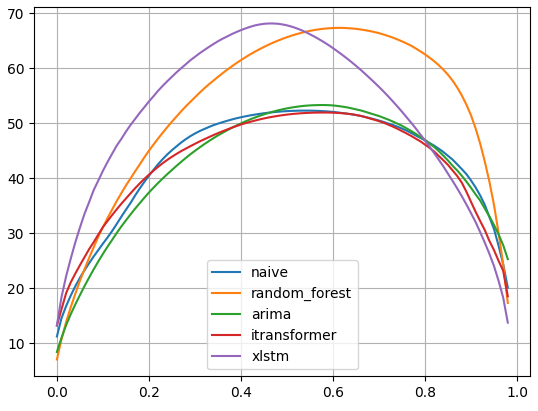
\includegraphics[width=\linewidth]{../images/results/quantile_pinball_scores.pdf}
  \caption{Quantile pinball scores for all models}
\end{subfigure}
\begin{subfigure}{0.45\textwidth}
  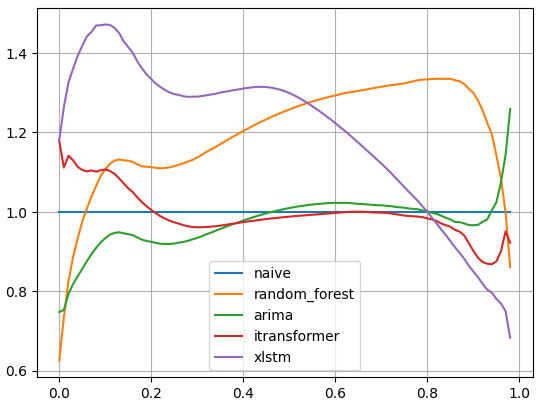
\includegraphics[width=\linewidth]{../images/results/quantile_pinball_scores_to_id1.pdf}
  \caption{Quantile pinball scores normalized based on naive}
\end{subfigure}
\caption{Quantile pinball scores for each model}
\label{Figure::pinball_scores}
\end{figure}


%Figure \ref{Figure::pinball_scores} shows the pinball scores for each quantile for each model.
%On the left the raw pinball scores are shown.
%The right graph shows the pinball score in relation to the pinball score of the naive model.
%These values are calculated by dividing the pinball score for each quantile $q$ for each model by the the pinball score for the quantile $q$ for the naive model.
%
%These charts show, that random forest performs the best on the lowest quantile and is among the best in the higher quantiles. 
%%Across most of the percentiles, from about $0.1$ to $0.8$ both random forest and xlstm have the worst pinball score.
%The xLSTM shines in the higher quantiles. 
%The pinball scores for xLSTM are the best in the higher percentiles. 
%This is in line with this model having the best RMSE, due to the nature of the otliers being very extreme.


%Figure \ref{Figure::Model_predictions} shows the predictions for the machine learning models on an example day and the actual imbalance price.

%\begin{figure}
%  \centering
%\begin{subfigure}{0.45\textwidth}
%  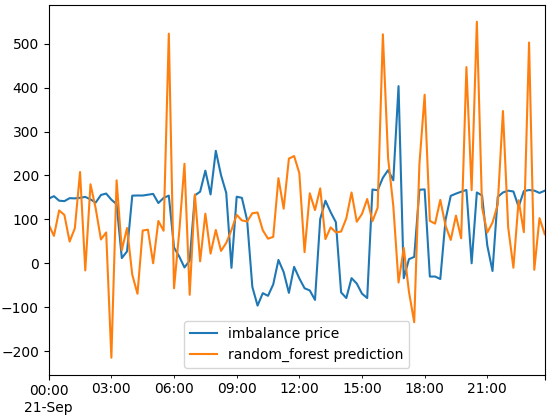
\includegraphics[width=\linewidth]{../images/results/random_forest_prediction.png}
%  \caption{Predictions of random forest}
%\end{subfigure}
%\begin{subfigure}{0.45\textwidth}
%  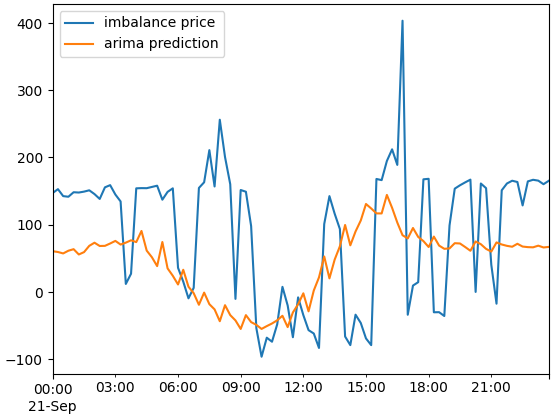
\includegraphics[width=\linewidth]{../images/results/arima_prediction.png}
%  \caption{Predictions of ARIMA}
%\end{subfigure}
%\begin{subfigure}{0.45\textwidth}
%  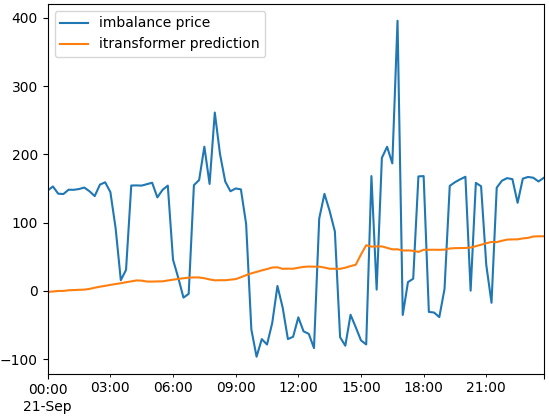
\includegraphics[width=\linewidth]{../images/results/itransformer_prediction.png}
%  \caption{Predictions of iTransformer}
%\end{subfigure}
%\begin{subfigure}{0.45\textwidth}
%  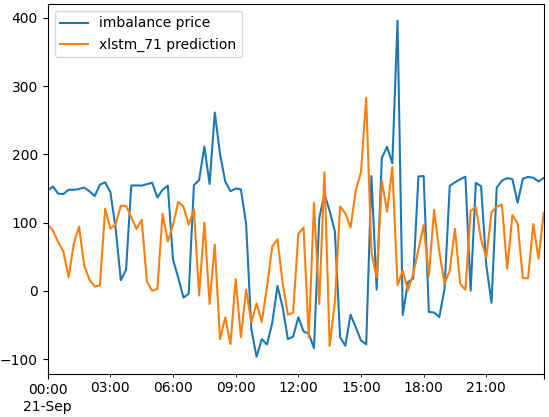
\includegraphics[width=\linewidth]{../images/results/xlstm_prediction.png}
%  \caption{Predictions of xLSTM}
%\end{subfigure}
%\caption{Predictions of the different models on example day}
%\label{Figure::Model_predictions}
%\end{figure}
%
%While random forest better predicticts the imbalance price with regards to mean average error, the xLSTM model seems to better capture outlieres, resulting in a lower mean %squared error.
%
%
\section{Different xLSTM block structures}

  \begin{table}[]
\centering
\begin{tabular}{l|l|l|l}
Configuration name 		&  RMSE 			 & MAE 			 & CRPS			\\\hline
xLSTM\_7\_1 4 seq		&$ 302.57\pm 6.68	$&$ \underline{84.33 \pm 1.17}	$&$ \underline{40.30	\pm0.24} $\\
xLSTM\_1\_0 96 seq		&$\underline{316.81\pm5.37} $&$ 85.68\pm 1.81	$& $40.34	\pm 0.32$\\
xLSTM\_1\_1 96 seq		&$ 318.48\pm12.03 	$&$87.73	\pm 3.16	$&$ 40.99	\pm 1.05$\\
xLSTM\_7\_1 96 seq	 	&$325.70 \pm5.56	$&$85.76\pm 2.09	$&$ 40.47	\pm 0.27$\\ 
\end{tabular}
\caption{Error metrics and CRPS for different xLSTM block configurations}
\label{Table::Performance_xLSTM}

\end{table}
\begin{table}
\centering
\begin{tabular}{l|l|l|l}
Configuration name 		& 50\%-cov 		& 90\%-cov 		& 98\%-cov \\\hline
xLSTM\_7\_1 4 seq	&$ 0.240 \pm 0.019	$&$ \underline{0.759 	\pm 0.012}	$&$ \underline{0.910 \pm 0.009}	 $\\
xLSTM\_1\_0 96 seq		&$\underline{ 0.277 \pm0.023}	$&$  0.743 \pm0.025	$&$ 0.886\pm0.028	$\\
xLSTM\_1\_1 96 seq		&$ 0.263 \pm0.046	$&$ 0.732 \pm0.044	$&$ 0.877\pm 0.032	$\\
xLSTM\_7\_1 96 seq	 	&$ 0.263 \pm0.021	$&$ 0.724 \pm0.014	$&$ 0.867 \pm0.010	$\\ 
\end{tabular}
\caption{Quantile metrics for different xLSTM block configurations}
\label{Table::Performance_xLSTM_quantile}
\end{table}
This experiment investigates how internal architectural choices in the xLSTM model — specifically the composition of mLSTM and sLSTM blocks — affect predictive performance. Tables \ref{Table::Performance_xLSTM} and \ref{Table::Performance_xLSTM_quantile} report the results for several variants, including the default 7\_1 configuration, as well as pure mLSTM (1\_0) and mixed (1\_1) structures. All models were trained with 96-step input sequences, except for the 7\_1 configuration with a short 4-step input, which serves as a reference for sequence length effects.

The results show that architectural variation has only a minor effect on forecasting performance. All 96-step configurations yield similar MAE (~85–88) and CRPS (~40.3–41.0), with no clear winner. The pure mLSTM model (1\_0) achieves the lowest RMSE (316.81) and best coverage (50\%-cov: 0.277), while the default mixed configuration (7\_1) performs slightly worse across all metrics.

Interestingly, the 4-sequence variant (7\_1) outperforms all 96-sequence models in both MAE (84.33) and CRPS (40.30), and reaches the highest coverage at the 90\% and 98\% levels. This suggests that shorter input sequences can yield sharper, more reactive forecasts, possibly by reducing over-smoothing and forcing the model to focus on the most recent dynamics. 

Overall, the results indicate that xLSTM performance is robust to architectural variation, and more sensitive to sequence length than to the internal mix of memory cell types.


\section{iTransformer variable sequence length}
This experiment investigates how the iTransformer model’s performance varies with different input sequence lengths. As shown in Tables \ref{Table::Performane_sequence_length} and \ref{Table::Performance_sequence_length2}, the model was evaluated using sequences of 4, 96, 192, and 384 time steps.

In terms of point forecast accuracy, longer input sequences do not lead to performance improvements. On the contrary, the shortest-sequence model (4 seq) achieves the lowest RMSE (200.19) and lowest MAE (139.87), despite having access to significantly less historical context. As sequence length increases, both MAE and RMSE deteriorate slightly, while CRPS increases notably, from 49.24 (4 seq) to 58.68 (384 seq).

This trend is even more pronounced in the quantile coverage metrics: the 4-sequence model attains the highest coverage across all levels (e.g. 90\%-cov = 0.841), while longer sequences exhibit steadily declining coverage, down to 0.282 at 90\% for the 384-step model. This suggests that longer sequence inputs lead the iTransformer to produce overconfident, underdispersed forecasts, which fail to reflect true uncertainty in imbalance price dynamics.

A possible explanation is that with longer inputs, the model tends to overfit to smoothed trends or ignore recent volatility, which reduces its responsiveness to short-term price spikes. 

Overall, these results imply that for the iTransformer architecture, shorter input sequences yield better-calibrated and more robust forecasts, particularly in capturing tail risk. This highlights a critical design consideration for sequence models: more historical context does not necessarily translate into better probabilistic performance — especially in volatile, regime-switching markets like imbalance pricing.

 \begin{table}[]
\centering
\begin{tabular}{l|l|l|l}
 Configuration name &  RMSE 		& MAE 			& CRPS \\\hline
iTransformer 4 seq    &$ 200.19 \pm 0.07	$&$ 139.87	\pm 0.06	$&$ \underline{49.24 \pm 0.04	}$ \\
 iTransformer 96 seq &$  \underline{186.15 \pm  0.12} $&$ \underline{135.78 \pm 0.06} $ &$  54.93\pm 0.02$\\
 iTransformer 192 seq &$ 188.02 \pm 0.01$ &$ 135.90 \pm 0.01$&$ 56.49 \pm0.13 $ \\
 iTransformer 384 seq &$ 188.16 \pm 0.58 $&$ 135.85 \pm 0.31 $&$ 58.68 \pm 0.11 $ \\
\end{tabular}
\caption{Error metrics and CRPS for different sequence lengths}
\label{Table::Performance_sequence_length}

\end{table}
\begin{table}
\centering
\begin{tabular}{l|l|l|l}
 Configuration name 	& 50\%-cov 		& 90\%-cov 		& 98\%-cov \\\hline
iTransformer  4 seq   	&$ \underline{0.356	\pm 0.001}$&$ \underline{0.841	\pm 0.000}	$&$\underline{0.959 \pm 0.000}	$ \\
 iTransformer 96 seq 	&$ 0.088 \pm 0.004$&$ 0.540 \pm 0.012$ 	&$ 0.755 \pm 0.003$ \\
 iTransformer 192 seq 	&$ 0.072 \pm 0.002$&$ 0.415\pm 0.016$ 	&$ 0.660 \pm 0.008$ \\
 iTransformer 384 seq 	&$ 0.049 \pm 0.002 $&$ 0.282 \pm 0.011$	&$ 0.475 \pm 0.030$\\
\end{tabular}
\caption{Quantile metrics for for different sequence lengths}
\label{Table::Performance_sequence_length2}
\end{table}



\section{iTransformer multiple target variables}

This experiment evaluates whether the iTransformer benefits from multi-target learning, i.e., jointly forecasting imbalance price along with additional target variables such as intraday indices, ENTSO-E physical data, and Netzregelverbund indicators. Table \ref{Table::Performance_targets} compares the predictive performance of models trained on different target combinations, including a combined configuration encompassing all auxiliary series.

Across all setups, no substantial performance improvements are observed. All variants achieve nearly identical RMSE (~185.5–186.0), MAE (~135.4–135.8), and CRPS (~54.8–54.9). Similarly, Table \ref{Table::Performance_targets2} shows minimal variation in quantile coverage metrics, with the combined model performing only marginally better at the 50\%-level (0.098) but showing no consistent gains at higher coverage levels.

These results suggest that the selected auxiliary targets — while related to the system state — do not provide additional predictive structure that improves the reBAP forecast. A likely reason is that these variables either correlate only weakly with the imbalance price or introduce noise that dilutes the learning signal for the main target.

Overall, this experiment indicates that multi-target learning does not enhance performance in this setting, and that focused single-target modeling may be preferable for probabilistic imbalance price forecasting — unless better-aligned or more informative auxiliary variables can be identified.

 \begin{table}[]
\centering
\begin{tabular}{l|l|l|l}
 Configuration name			&  RMSE 			& MAE 			& CRPS 			 \\\hline
 iTransformer intraday indices 		&$ 185.95\pm 0.46	$&$ 135.67 \pm 0.30	$&$ 54.84\pm0.17	$\\
 iTransformer entsoe data		&$  185.95 \pm 0.38 $&$ 135.65 \pm 0.19		$&$ 54.93 \pm 0.011		 $\\
 iTransformer netzregelverbund 	& $186.05 \pm 0.35	$&$ 135.80\pm0.27	$&$ 54.90\pm 0.02	$\\
 iTransformer combined 		&$ \underline{185.52 \pm 0.93}	$&$ \underline{135.36\pm 0.61}	$&$ \underline{54.81\pm 0.18	2} $\\
\end{tabular}
\caption{Error metrics and CRPS for multiple target variables}
\label{Table::Performance_targets}
\end{table}
\begin{table}
\centering
\begin{tabular}{l|l|l|l}
 Configuration name			& 50\%-cov 		& 90\%-cov 		& 98\%-cov \\\hline
 iTransformer intraday indices 		&$0.090\pm 0.009	$& $0.546\pm 0.011	$ & $0.755 \pm 0.002$\\
 iTransformer entsoe data		&$0.090 \pm  0.002	$&$ 0.533 \pm 0.004	$&$0.755 \pm 0.006 $\\
 iTransformer netzregelverbund 	&$0.085\pm 0.004	$&$\underline{0.551 \pm 0.010}	$&$ 0.750 \pm 0.003$\\
 iTransformer combined 		&$ \underline{0.098\pm 0.015}	$&$ 0.542 \pm 0.018 	$&$ \underline{0.755 \pm 0.003}$\\
\end{tabular}
\caption{Quantile metrics for for  multiple target variables}
\label{Table::Performance_targets2}
\end{table}


%\begin{figure}
% % \centering
%\begin{subfigure}{0.45\textwidth}
%  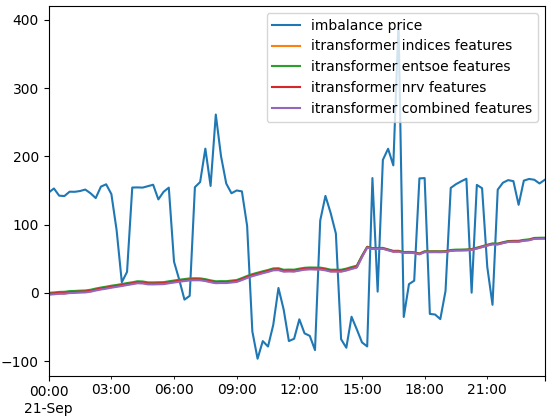
\includegraphics[width=\linewidth]{../images/results/itransformer_target_variables_aep.png}
%  \caption{Predictions of models with imbalance price}
%\end{subfigure}
%\begin{subfigure}{0.45\textwidth}
%  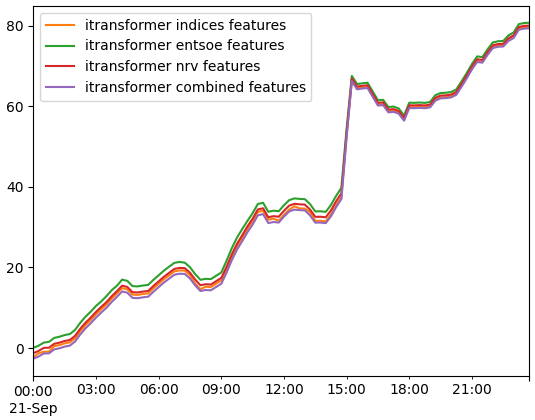
\includegraphics[width=\linewidth]{../images/results/itransformer_target_variables_alone.png}
%  \caption{Predictions of models without imbalance price}
%\end{subfigure}
%\caption{Predictions of iTransformers trained on multiple target variables}
%\label{Figure::Targets_prediction}
%\end{figure}


\section{iTransformer different prediction horizons}
This experiment explores whether training the iTransformer to forecast longer horizons improves its ability to predict the one-hour-ahead imbalance price. The model was trained with forecast horizons of 4, 12, 24, 48, and 96 steps, and evaluated solely on the one-hour-ahead target.

As shown in Tables \ref{Table::Performance_targets_horizon} and \ref{Table::Performance_targets_horizon2}, all configurations perform nearly identically. Differences in RMSE, MAE, and CRPS across horizons are minimal (less than 0.3 points in each metric), and quantile coverage metrics vary only in the third decimal place. The longest-horizon model (96 steps) does not outperform shorter-horizon models — in fact, it shows slightly worse MAE (135.99) and CRPS (54.94), though the differences are insignificant.

These results suggest that longer forecast horizons do not yield any benefit for short-term imbalance price prediction in this setup. A likely explanation is that the model is trained to optimize the entire sequence output, which can dilute the learning focus on the one-hour-ahead value. Additionally, longer sequences may introduce training complexity without additional relevant signal.

This experiment implies that training the model specifically for the target horizon is sufficient, and that increasing the output range does not lead to generalization gains

 \begin{table}[]
\centering
\begin{tabular}{l|l|l|l}
 Configuration name			&  RMSE 			& MAE 			& CRPS 	\\\hline
 iTransformer 4 horizon		& $\underline{186.16 \pm 0.02}	$&$ 135.79 \pm 0.03	$&$54.92 \pm 0.01$\\
 iTransformer 12 horizon		&$ 186.24\pm 0.11	$&$135.89 \pm 0.14	$&$54.89 \pm 0.02$ \\
 iTransformer 24 horizon		&$ 186.17	\pm 0.01	$&$ \underline{135.76 \pm 0.03}	$&$54.89	\pm 0.01$\\
 iTransformer 48 horizon		&$ 186.22  \pm 0.03	$&$\underline{ 135.76 \pm 0.04	}$&$\underline{54.88	\pm 0.00}$ \\
 iTransformer 96 horizon		&$ 186.47	\pm 0.01	$&$ 135.99 \pm 0.02	$&$54.94	\pm 0.00$\\
\end{tabular}
\caption{iTransformer performance for multiple target variables}
\label{Table::Performance_targets_horizon}
\end{table}
\begin{table}
\centering
\begin{tabular}{l|l|l|l}
 Configuration name			&   50\%-cov 		& 90\%-cov 		& 98\%-cov \\\hline
 iTransformer 4 horizon		&$\underline{0.086 \pm 0.001}	$&$ 0.541\pm 0.003 	$&$\underline{0.756 \pm 0.001}$\\
 iTransformer 12 horizon		&$0.084\pm 0.002	$&$ \underline{0.549\pm 0.009}	$ &$ 0.753 \pm 0.003$ \\
 iTransformer 24 horizon		&$0.084\pm 0.001	$&$0.543\pm 0.002	 $&$0.755 \pm 0.001$\\
 iTransformer 48 horizon		&$0.085\pm 0.001	$&$ 0.543\pm 0.002	 $&$\underline{ 0.756\pm 0.001}$ \\
 iTransformer 96 horizon		&$0.083\pm 0.000	$&$ 0.544\pm 0.001	 $&$ \underline{0.756 \pm 0.000}$\\
\end{tabular}
\caption{iTransformer performance for multiple target variables}
\label{Table::Performance_targets_horizon2}
\end{table}

%\begin{figure}
%  \centering
%\begin{subfigure}{0.45\textwidth}
%  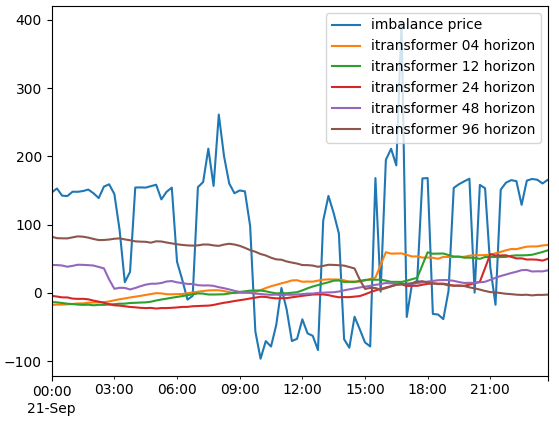
\includegraphics[width=\linewidth]{../images/results/itransformer_horizon_lengths.png}
%  \caption{Predictions of models with imbalance price}
%\end{subfigure}
%\begin{subfigure}{0.45\textwidth}
%  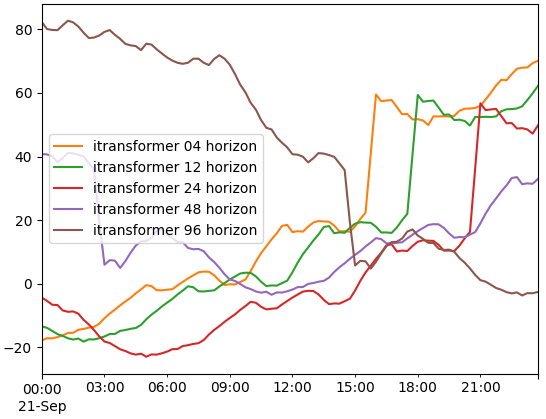
\includegraphics[width=\linewidth]{../images/results/itransformer_horizon_lengths_alone.png}
%  \caption{Predictions of models without imbalance price}
%\end{subfigure}
%\caption{Predictions of iTransformers trained on different forecasting horizons}
%\label{fig:fig}
%\end{figure}


\section{Feature Importance: Insights from Random Forest}
\label{Section::Analysis or Evaluation of Something}    


Table  \ref{Table::Feature_importance} lists the 15 most important input features used by the Random Forest model, aggregated across time-shifted variants. The top-ranked features are dominated by market price signals, most notably the hourly spot price and IDA1, which stand out with clearly higher importance values than the rest. This underscores the strong influence of recent and forward market indicators in reBAP prediction.

Subsequent features — including lagged intraday indices (IDFULL, ID3, ID1), the AEP schätzer, and fossil generation metrics (hard coal, lignite) — show a more gradual decline in importance, suggesting that a moderately wide set of features contributes meaningfully to the model’s performance. In particular, forecasted residual load stands out over shifted or error-based versions, indicating that forward-looking demand-supply imbalances are more informative than retrospective deviations.

Weather-related variables such as temperature at 1m depth, wet temperature, and wind offshore forecast error also appear in the top 15. The presence of forecasting errors over raw values for wind points to the importance of uncertainty signals from volatile renewables.

Overall, the results suggest that the Random Forest relies on a core set of market-driven features, supported by operational and meteorological indicators. Rather than focusing on a narrow subset, the model balances high-impact features with a broader context, reflecting the multifactorial nature of imbalance price formation.



%Table \ref{Table::Feature_importance} contains information about the most important features for the random forest prediction.
%The top 6 most important features consist of information about prices. Interesting is, that the intraday index shifted by one day still has a very high feature importance.
%The next two most important features \textit{lignite actual generation shifted by 30 minuts} and \textit{fossil hard coal actual generation shifted 30 minutes} contain %information about generated energy provided by fossil energy sources.
%The third features containing information about fossil energy sources ranks 14\textsuperscript{th} most important. 
%The importance of features doesn't change much after the  10\textsuperscript{th} most important feature.
%Out of the wheather data the temperature was the most important, followed by the difference in forecast for the solar radiation within one hour.
%Notable information from this importance is that the forecasted residual load is more important to the model than the shifted actual residual load or the shifted forecasting %error.
%For solar and wind offshore generation the opposite is true. 
%The shifted forecasting error is more important than both the forecast and the shifted actual measurement.

\begin{table}[]
\centering
\begin{tabular}{l|l|l}
 Feature rank & Parameter & Importance \\\hline
 1-5 & Hourly spot price& 0.0970\\
 6-9, 14& IDA1&0.0582 \\
 12, 15, 16, 17, 40&intraday IDFULL shifted 1 day & 0.0306 \\
 10, 19, 21, 26, 32  &aep schaetzer shifted 30 minutes&0.0303\\
 11, 20, 24, 25, 29 &intraday ID3 shifted 1 day &0.0283\\
 13, 18, 22, 23, 69 & intraday ID1 shifted 1 day &0.0271\\
 27, 28, 31, 46, 71 & entsoe fossil hard coal actual generation & 0.0203\\
 30, 34, 35, 36, 39 & entsoe lignite actual generation & 0.0196 \\
 33, 37, 41, 48, 66 & forecasted residual load & 0.0177 \\
 38, 51, 52, 85, 98 & entsoe wind onshore actual & 0.0154 \\
42, 57, 65, 75, 80 & entsoe fossil gas actual generation & 0.0151 \\
44, 61, 63, 70, 141 & dwd measurements temperatur in 1m depth & 0.0145 \\
55, 62, 67, 87, 93 & dwd measurements wet temperature & 0.0143 \\
58, 76, 81, 101, 118 & wind offshore forecasting error & 0.0135 \\
 
\end{tabular}
\caption{15 most important features of random forest sorted from most important to least important. For each feature all shifted values are aggregated to get the importance.}
\label{Table::Feature_importance}
\end{table}


\end{document}
